\documentclass[a4paper,10pt]{article}
\usepackage[fleqn]{amsmath}
\usepackage{amsfonts}
\usepackage{amssymb}
\usepackage{theoremref}
\usepackage[pdftex]{hyperref}
\usepackage{daa}
\usepackage{listings}
\usepackage{tikz}
\usetikzlibrary{arrows,decorations.pathmorphing,backgrounds,positioning,fit,petri}



\hypersetup{colorlinks,%
		citecolor=black,%
		filecolor=black,%
		linkcolor=black,%
		urlcolor=blue}

\title{\textbf{Hive}\\ Sistema Distribuido para la paralelización de tareas}
\author{Carlos David Muñiz Chall\\Jesús Manuel Garnica Bonome}
\date{}

\begin{document}
	\maketitle

	\section{Descripción}
		
		El objetivo de este sistema es ejecutar un gran volumen de trabajo usando, las capacidades de paralelización propias a una red de computadoras e interactuar con los clientes como una única entidad. Como prestaciones adicionales se tienen la extensibilidad automatica de la red y una alta tolerancia a fallos basada en la replicación de tareas.
		El sistema ejecutará cualquier tipo de tarea, simpre que esta cumpla los requisitos definidos en \textbf{Uso y definición de tareas}[\ref{sec_task}] .
		
		Hive \textbf{no brinda} proteción contra ataques o uso malicioso de algún componente dado que su diseño supone un entorno amigable.
		
	\section{Arquitectura}
		El diseño de componentes y funcionalidades está basado en una arquitectura \textbf{superpeer}\cite{Tanenbaum}, esta puede ser entendida como un arquitectura \textbf{cliente-servidor}, donde el servidor es un sistema distribuido \textbf{peer-to-peer}. Los nodos miembros de este subsistema manejan la distribución de las tareas que deben ejecutar los nodos clientes, para organizar la replicación de tareas y el balance de carga, se encuentran enlazados en un anillo, donde cada nodo conoce a su siguiente y su anterior.\\		
					
		En su conjunto el sistema consta de dos tipos de nodos:	
		\begin{itemize}
			\item Drone: nodos correspondientes a la parte cliente, en estos es donde se realiza el procesamiento de las tareas.
			
			\item Overlord: miembros de la red \textbf{peer-to-peer} que constituye el servidor, estos realizan el balance de carga y la replicación de las tareas.			
		\end{itemize}
		
		\begin{figure}[h]
			\centering
			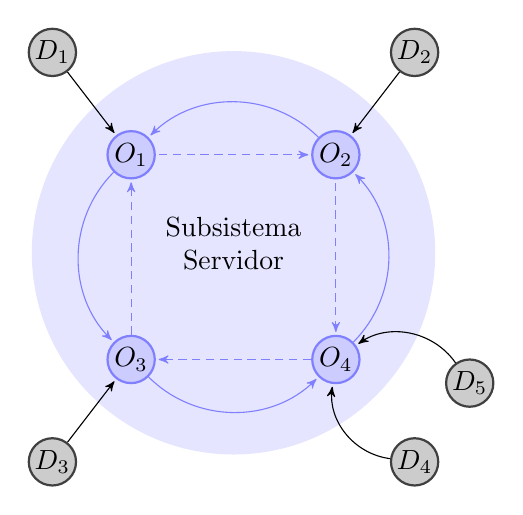
\begin{tikzpicture}
			[node distance=1.3cm,>=stealth',on grid,bend angle=45,auto,
			overlord/.style={circle,draw=blue!50,fill=blue!20,thick,inner sep=0pt,minimum size=6mm},		
			drone/.style={overlord,draw=black!75,fill=black!20},
			every label/.style= {red}]
			
			\node [overlord](o1)                                 {$O_1$};
				\node (fo1) [right=of o1, yshift=3mm]            {};
				\node (fo3) [below=of o1, xshift=-3mm]           {};
				
			\node [overlord](o2) [right=of fo1, yshift=-3mm]     {$O_2$}
				edge             [post,bend right, draw=blue!50] (o1)
				edge             [pre, draw=blue!50, densely dashed] (o1);
			    \node (fo2) [below=of o2, xshift=3mm]            {};
				
			\node [overlord](o3) [below=of fo3, xshift=3mm]      {$O_3$}
				edge             [pre,bend left, draw=blue!50]   (o1)
				edge             [post, draw=blue!50, densely dashed]   (o1);	
						
			\node [overlord](o4) [below=of fo2, xshift=-3mm]     {$O_4$}
				edge             [pre,bend left, draw=blue!50]   (o3)
				edge             [post, draw=blue!50, densely dashed]   (o3)
				edge             [post,bend right, draw=blue!50] (o2)
				edge             [pre, draw=blue!50, densely dashed] (o2);
			
			
			\node [drone](d1) [above=of o1, xshift=-10mm] {$D_1$}
				edge [post] (o1);
			\node [drone](d2) [above=of o2, xshift=10mm] {$D_2$}
				edge [post] (o2);
			\node [drone](d3) [below=of o3, xshift=-10mm] {$D_3$}
				edge [post] (o3);
			\node [drone](d4) [below=of o4, xshift=10mm] {$D_4$}
				edge [post,bend left] (o4);
			\node [drone](d5) [above=of d4, xshift=7mm, yshift=-3mm]  {$D_5$}
				edge [post,bend right] (o4);			
			
			\begin{scope}[on background layer]
				\node (r1) [circle,fill=blue!10,rounded corners,fit=(o1)(o2)(o3)(o4)(fo1)(fo2)(fo3)] {Subsistema \\ Servidor};
			\end{scope}
			
			
			\end{tikzpicture}
			\caption{Esquema general de un sistema Hive, Drones = {$D_1$,$D_2$,$D_3$,$D_4$,$D_5$} Overlords = {$O_1$,$O_2$,$O_3$,$O_4$} }
		\end{figure}		
		
		\pagebreak
		\subsection{Balance de Carga}			 
			
			Cada $overlord$ perteneciente al sistema está a cargo de varios $drones$, los cuales solicitan o generan tareas, cada vez que un $drone$ se encuentra libre de trabajo, porque termino la tarea asignada o está a la espera del resultado de una subtarea, solicita una nueva tarea al $overlord$ asignado.
			
			El balance de carga se logra con dos procesos diferentes, el primero consiste en distribuir lo más equitativamente posible los $drones$ entre la población de $overlords$, para esto cada uno mantiene un campo \textbf{salto de carga} que es la cantidad de nodos hacia adelante que se pasará al próximo $drone$ que solicite un responsable, luego de cada solicitud este campo es aumentado en $1$ hasta que llege al tamaño del anillo, momento en el que vuelve a $0$.
			
			El otro proceso tiene lugar cuando un $overlord$ no puede responder a la solicitud de tareas, porque él mismo no posee ninguna, en este momento se replica la mitad de las tareas pendientes del primer $overlord$, en el sentido normal del anillo, que tenga alguna o se le reponde al $drone$ que intente de nuevo luego de esperar un tiempo determinado.
		
		\subsection{Tolerancia a Fallos}
			La confiabilidad se basa en la replicación de las tareas, de modo que ninguna tarea este almacenada en un solo nodo del sistema, una caracteristica importante es que tanto el codigo como los datos asociados a una tarea son inmutables, por lo que no es necesario ningún protocolo especial para la consistencia de las replicas.
			
			La replicación ocurre en dos momentos diferentes, al ser recibida la tarea por un $overlord$ y cuando este la entrega a los nodos que supervisa. Cuando una tarea es recibida por el $overlord$ este lanza una solicitud de replicación dentro del subsistema servidor, con esto se logra que si se pierde el nodo que recibió la tarea, sin que esta halla sido asignada a ningún $drone$, la tarea no se pierda pues las replicas se encuentran disponibles en otros $overlords$. Después de la replicación la tarea es insertada en una cola en los $overlords$ que la hallan recibido, la segunda replicación ocurre cuando un $drone$ solicita una tarea, la que esta al principio de la cola se le es asignada, pero no es eliminada hasta que no haya sido asignada a un número determinado de $drones$, para evitar que el fallo de un $drone$ en conjunto con el fallo de varios $overlords$ impida la realización de algún trabajo.

			Debido a la replicación la pérdida inesperada de un nodo, sin importar su tipo, no afecta el funcionamiento del sistema, pero hay dos casos que requieren una consideración más profunda; primero, si pierde un $overlord$ las tareas no se afectan, pero la estructura de anillo si, en este caso se usan las referencias que tiene cada miembro del anillo hacia el anterior para descubir los dos nodos que deberían estar enlazados al que se perdió, y enlazando estos dos se recupera la estructura nuevamente; segundo, si el nodo perdido es el nodo cliente de la tarea original, no una subtarea generada por esta, el sistema no puede entregar el resultado del cómputo solicitado, pero esto se considera responsabilidad del cliente. 
	
	\section{Protocolo Hive}
	
		Para garantizar la extensibilidad del sistema se considera nodo del mismo a cualquier proceso que siga el protocolo que se expondrá a continuación.
		
		Como la mayor parte de dicho protocolo descansa sobre \textbf{RPC}\cite{rpc}, las acciones se definirán en términos de argumentos y resultados. Para lograr la interacción a través de rpc cada nodo debe mantener un servidor rpc operacional mientras esté activo, la dirección a donde esté sujeto será considerada la dirección del nodo dentro de la red. En este servidor se deben registrar las funciones que se describen para cada tipo de nodo.
		
		Las acciones que puedan demorar más que una simple comfirmación de llegada, aparecen como una pareja de funciones, una en el destino para iniciar la acción y una en el origen para recibir los resultados, minimizando la posibilidad de que un procesamiento lento sea confundido con un error de comunicación. 
		
		Las próximas secciones describen el protocolo, separando las acciones por las interfaces de comunicación a la que pertenecen.
	
		%TODO: definir tarea y datos
	\pagebreak
	\subsection{Overlord-Overlord}
		\subsubsection{EnterRing}\label{entring}
			Esta acción es iniciada por un nodo que no pertenece al anillo de $overlords$ con el objetivo de incluirse.
			\\
			\textbf{Argumentos:} dirección del nodo que desea unirse. \\
			\textbf{Resultados:} (dirección del nodo próximo, nombre para el nuevo nodo del anillo)\\
			
			El nodo que responde tiene la responsabilidad de informar su nodo próximo que su anterior ya no es él, sino el nuevo nodo, además de modificar sus propias direcciones consistentemente.
			Quien inicia la acción queda incluido en el anillo con antecesor el nodo al que envió la solicitud y como sucesor el sucesor de este último, si este nodo ya posee un nombre el de la respuesta debe ser ignorado.
			
		\subsubsection{SetPredecessor}\label{setpre}
			Informa al nodo receptor que su antecesor ha cambiado.
			\\
			\textbf{Argumentos:} dirección del nodo que será el nuevo antecesor. \\
			\textbf{Resultados:} \textbf{ACK}\\
			
		\subsubsection{Address}\label{addr}
			Informa al receptor el resultado de la solicitud de resolucion de dirección.
			\\
			\textbf{Argumentos:} (a: dirección del nodo solicitado, i: identificador único de solicitud)\\
			\textbf{Resultados:} \textbf{ACK}\\
			Esta acción es la forma de recibir los resultados de \textbf{Who}[\ref{who}], el identificador es único para cada solicitud iniciada por un nodo, no necesita ser único en todo el sistema
		
		\subsubsection{Who}\label{who}
			Operación de resolución de direcciones dentro del anillo.
			\\
			\textbf{Argumentos:} (c: contador, a: dirección del nodo que inicio la acción \textbf{Who}, i: identificador único de solicitud)\\
			 \textbf{Resultados:} \textbf{ACK}\\
			
			\begin{itemize}
				\item $c > 0$: se envia \textbf{Who(c - 1, a, i)} al próximo nodo en el sentido normal del anillo.
				\item $c = 0$: se envia \textbf{Address(a, i)}[\ref{addr}] al nodo con dirección \textbf{a}.
				\item $c < 0$: si el nodo antecesor es accesible se envia \textbf{Who(c, a, i)} al nodo antecesor, si este no es accesible se envia \textbf{SetPredecessor(dirección del nodo actual)}[\ref{setpre}] al nodo con dirección \textbf{a}
			\end{itemize}
			
		\subsubsection{Replicate}\label{rep}
			Ordena la replicación de una tarea dentro del anillo.
			\\
			\textbf{Argumentos:} (t: tarea, sf: factor de salto, sc: contador de saltos, rc: contador de replicaciones)\\
			\textbf{Resultados:} \textbf{ACK}\\
			
			\begin{itemize}
				\item $sc = 0$: se adiciona \textbf{t} a la cola de tareas del $overlord$ actual.
					\begin{itemize}
						\item $rc > 0$: se envia \textbf{Replicate(t, sf, sf, rc - 1)} en el sentido normal del anillo.
					\end{itemize}
				\item $sc > 0$: se envia \textbf{Replicate(t, sf, sc - 1, rc)} al siguiente nodo del anillo.			
			\end{itemize}
			
		\subsubsection{Consume}\label{cons}
			Fuerza la replicación de tareas hacia un $overlord$ que no posee ninguna
			\\
			\textbf{Argumentos:} a: dirección del overlord que inicio la acción \textbf{Consume}\\
			\textbf{Resultados:} \textbf{ACK}\\
			
			Si no el nodo no posee ninguna tarea pasa la solicitud al nodo siguiente en el anillo, si él es el que inicio la acción, se espera un tiempo determinado antes de repetirla. En caso de tener tareas pendientes y no ser el nodo que inicio la acción se ejecuta una serie de acciones \textbf{PutTask}[\ref{ptask}] hacia el nodo con dirección \textbf{a}.
			
	\pagebreak	
	\subsection{Overlord-Drone}
		\subsubsection{PutTask}\label{ptask}
			Recibe una tarea. Esta acción es implementada por ambos tipos de nodos.
			\\
			\textbf{Argumentos:} t: tarea\\
			\textbf{Resultados:} \textbf{ACK}\\
			
			\begin{itemize}
				\item $Drone$: \linebreak
					Esta acción es el resultado de haber invocado \textbf{GetTask}[\ref{gtask}] en un $overlord$, la tarea asignada es preparada para ejecutarse cuando el $drone$ esté libre de trabajo.
				\item 	$Overlord$: \linebreak
					Puede ser tando el resultado de una acción \textbf{Consume}[\ref{cons}], en cuyo caso se recibirán las replicas cada una en una invocación diferente de \textbf{PutTask}, o ser la solicitud de un $drone$ cliente de iniciar una nueva tarea o subtarea. La tarea \textbf{t} es añadida a la cola de tareas y su replicación es iniciada[\ref{rep}].
			\end{itemize}	
			
		\subsubsection{GetTask}\label{gtask}
			Esta acción es implementada solo por los $overlords$, su invocación señaliza que un drone está listo para recibir una nueva tarea.
			\\
			\textbf{Argumentos:} a: dirección del $drone$ que solicita la tarea\\
			\textbf{Resultados:} \textbf{ACK}\\
			
			La respuesta a esta acción es enviada a través de \textbf{PutTask}[\ref{ptask}], la tarea que se envia es la del principio de la cola, esta tarea es eliminada de la cola depués en un número determinado de invocaciones de \textbf{PutTask} que la contengan.
		
		\subsubsection{Hello}\label{hll}
			Inicio del proceso de inscripción de un $drone$ en el sistema, aunque es implentada por ambos tipos de nodos tiene significados diferentes, pues la inscripción de un $overlord$ en el anillo se realiza mediante \textbf{EnterRing}[\ref{entring}]
			\\
			\textbf{Argumentos:} a: dirección de un nodo en la red \\
			\textbf{Resultados:} \textbf{ACK}\\
			\begin{itemize}
				\item $Drone$: \linebreak
				Esta es la respuesta de un $overlord$ a una acción \textbf{Hello}, \textbf{a} es la dirección del $overlord$ que será responsable del $drone$ actual.
				\item $Overlord$: \linebreak
				El $overlord$ inicia una búsqueda usando \textbf{Who}[\ref{who}], para encontrar el $overlord$ que está a una distancia determinada de él, una vez que llege el resultado de la resolución de dirección esta es comunicada al drone con dirección \textbf{a} invocando \textbf{Hello} en él. La distancia que debe viajar \textbf{Who} aumenta con cada invocación de \textbf{Hello} hasta que pase por el nodo que inicio la búsqueda, en este caso la distancia vuelve a empezar en $0$.
			\end{itemize}
			
		\subsubsection{Register}\label{regt}
			Segunda etapa del proceso de inscripción de un $drone$ en el sistema, implementada únicamente por los $overlords$
			\\
			\textbf{Argumentos:} a: dirección del $drone$ a registrar\\
			\textbf{Resultados:} (aa: dirección del $overlord$ antecesor del que recibe el pedido, ap: dirección del sucesor, n: nombre para el $drone$)\\
			
			Al recibir la respuesta el $drone$ queda vinculado al $overlord$ que responde y posee las direcciones del antecesor y sucesor de este como alternativas en el caso de la pérdida del supervisor, si la conexión con los tres $overlords$ se pierde, el proceso de inscripción debe repetirse desde el principio. Un $drone$ que esté restableciendo su conexión con el subsistema servidor debe ignorar el campo del nombre en la respuesta y utilizar el asiganado la primera vez que se conectó.
			Cada $overlord$ debe garantizar que asigna nombres únicos a cada $drone$, sin importar que este vaya a ser ignorado.
			
	\pagebreak
	\subsection{Drone-Drone}
		\subsubsection{TaskResult}\label{tresult}
			Comunica la respuesta de una tarea.
			\\
			\textbf{Argumentos:} (t\_id: identificador de la tarea cuya respuesta se está transmitiendo, d: datos de la respuesta)\\
			\textbf{Resultados:} \textbf{ACK}\\
			
			Si el $drone$ donde se invoca este procedimiento ya tiene un resultado para la tarea con el identificador transmitido, esta respuesta será ignorada.
			
	\subsection{Descubrimiento de Nodos}
		Para comenzar a prestar servicio un nodo debe registrarse en el sistema, esto es conocer la dirección de un $overlord$ que esté registrado en el anillo y comenzar con \textbf{Hello}[\ref{hll}] hacia él en el caso de un $drone$, y en el caso de un $overlord$ iniciar \textbf{EnterRing}[\ref{entring}].
		 
		Un nodo puede obtener la dirección de un $overlord$ de dos formas, que el usuario que esta adicionando el proceso al sistema la provea, o realizar una búsqueda automática. Para la segunda se provee de soporte a nivel de mensajes \textbf{UDP}.
		
		Cada nodo ya registrado debe mantener un puerto \textbf{UDP} respondiendo a cualquier mensaje, con la dirección del $overlord$ en el cual está registrado, si es un $drone$, o con su propia dirección si es un $overlord$.
		
		El nodo que desea incorporarse debe utilizar mensajes de \textbf{broadcast} en su subred hasta obtener una dirección valida. La obtención automática de esta dirección podría ser imposible, cuando en la subred no existe ningún nodo registrado, en este caso el usuario debe proveer la dirección de algún nodo.
		
		Si un nodo es desconectado de la red por pérdida de los nodos a los que está enlazado, debe iniciar este proceso para descubrir un nuevo punto de enlaze.
		
		El puerto por el cual se efectua el descubrimiento puede variar, para permitir que varios sistemas disjuntos convivan en las mismas subredes.
		
	\section{Uso y Definición de Tareas}\label{sec_task}
		
		Para tabajar con Hive es necesario proveer el código y los datos de cada tarea. Por tarea se entiende cualquier $scrip$ en \textbf{Python} que cumpla las siguientes condiciones:
		\begin{itemize}
			\item No importa ningún módulo o paquete que no pertenezca a la biblioteca estandar o sea "tasksupport.py", que es el módulo por el cual se exponen los servicios de control de tareas e importación de dependencias.
			\item En el caso de que importe "tasksuppor.py", no modifica ninguna variable privada, aquellas cuyo nombre comienze por '\_'.
			\item (opcional) Antes de finalizar devuelve el resultado del cómputo a través de "tasksupport.CurrentTask.finalize(result)", de lo contrario se considera que la tarea finalizó sin ningún resultado, lo cual no es un error
			\item (opcional)  Para importar dependencias utiliza "tasksupport.import(dependence)", para cualquier otra forma de importar no se tienen garantias de que funcione.
		\end{itemize}
		
		Las dependencias pueden ser cualquier archivo valido para importar desde \textbf{Python}, estas deben ser proveidas desde la orden de ejecución de una tarea y deben incluir los $scrips$ con el codigo de las subtareas, en caso de tenerlas, y las dependencias de las mismas.

	%\subsection{Ciclo de Vida de una Tarea}
	
	\bibliography{sources}
	
\end{document}